% ISWC 2026 In-Use Track — LNCS format
\documentclass[runningheads]{llncs}

\usepackage{booktabs}
\usepackage{subcaption}
\usepackage{xcolor}
\usepackage{tikz}
\usetikzlibrary{positioning,arrows.meta,fit,backgrounds,calc}
\usepackage{listings}
\usepackage{hyperref}
\usepackage{graphicx}
\usepackage{amsmath}

\lstset{
  basicstyle=\ttfamily\small,
  keywordstyle=\bfseries,
  breaklines=true,
  frame=none,
  columns=flexible,
  aboveskip=4pt,
  belowskip=4pt,
}

\begin{document}

\title{Federated Biomedical Knowledge Graphs at Scale:\\
Graph-Native Storage, Cross-KG Queries, and AI-Agent Integration}

\author{Madhulatha Mandarapu\inst{1} \and
Sandeep Kunkunuru\inst{1}}

\authorrunning{M. Mandarapu and S. Kunkunuru}

\institute{VaidhyaMegha Private Limited, Hyderabad, India\\
\email{\{madhulatha,sandeep\}@samyama.ai}}

\maketitle

\begin{abstract}
We present Samyama, a graph database deployed in production for
federated biomedical knowledge graph analytics.  The system loads
ten public-health and biomedical knowledge graphs---137~million nodes
and 1.22~billion edges from sources including PubMed/MEDLINE,
ClinicalTrials.gov, FAERS, OMOP, DrugBank, UniProt, Reactome, and
WHO---into a single multi-tenant instance on commodity hardware.
Cross-KG federation is achieved through \emph{bridge properties} on
shared entities (genes, drugs, country codes, clinical terminologies),
enabling standard OpenCypher queries that span molecular biology,
clinical trials, adverse events, and population health without ETL
merging or schema-alignment middleware.

The engine is implemented in Rust with a graph-native query planner
that exploits adjacency-list statistics for direction-aware traversal
and an \texttt{ExpandInto} operator for bound-bound edge checks.
Version~1.0 introduces MVCC transaction isolation, adjacency-aware
aggregation (reading neighbor counts from the index instead of
scanning edges), and a streaming executor with early termination.

On a 500-query mega benchmark spanning all ten knowledge graphs,
Samyama achieves \textbf{500/500 (100\%)} correct answers---468 with
non-empty result sets and 32 returning zero rows due to documented
corpus-coverage gaps, not engine failures.  Each KG is additionally
exposed to LLM agents via the Model Context Protocol (MCP) with
domain-specific tool definitions, achieving 98\% accuracy on
biomedical questions versus 75\% for standalone GPT-4o.

\keywords{Knowledge graphs \and Biomedical data integration \and
  Graph databases \and OpenCypher \and Federation \and
  Model Context Protocol}
\end{abstract}

%% ================================================================
\section{Introduction}\label{sec:intro}

Biomedical knowledge is fragmented across dozens of public databases,
each covering a narrow slice of the translational research pipeline:
protein--protein interactions (STRING~\cite{szklarczyk2023string}),
biological pathways (Reactome~\cite{gillespie2022reactome}), drug--gene
interactions (DGIdb~\cite{freshour2021dgidb}), side effects
(SIDER~\cite{kuhn2016sider}), bioactivity assays
(ChEMBL~\cite{zdrazil2024chembl}), clinical trials
(ClinicalTrials.gov), post-market adverse events
(FDA FAERS), patient-level observational data (OMOP~\cite{hripcsak2015omop}),
protein sequences (UniProt~\cite{uniprot2023}), and
population-health indicators (WHO, World Bank).

Answering a question such as \emph{``For drugs in Phase~3 breast cancer
trials, what are their known adverse events in FAERS and which
biological pathways do their targets participate in?''} today requires
joining across at least four databases with ad-hoc scripting,
identifier reconciliation, and no transactional guarantees.

We present Samyama, a graph database system deployed in production
for federated biomedical knowledge graph analytics.  Our contributions
are:

\begin{enumerate}
\item \textbf{Ten-KG biomedical ecosystem} (Section~\ref{sec:kgs}).
  Ten complementary knowledge graphs---spanning molecular biology
  through population health---loaded into a single graph engine and
  federated via bridge properties on shared entities, requiring zero
  schema-alignment middleware.

\item \textbf{Graph-native query engine at billion-edge scale}
  (Section~\ref{sec:engine}).  A Rust-based engine with late
  materialization, a cost-based planner exploiting adjacency-list
  statistics, MVCC transaction isolation, and adjacency-aware
  aggregation---running 137M~nodes and 1.22B~edges on a single
  commodity server.

\item \textbf{500-query mega benchmark at 100\% pass rate}
  (Section~\ref{sec:eval}).  A comprehensive evaluation across all
  ten KGs with a transparent oracle that separates engine capability
  from corpus coverage.

\item \textbf{MCP-based AI-agent integration}
  (Section~\ref{sec:mcp}).  Domain-specific tool definitions that
  expose each KG to LLM agents, achieving 98\% accuracy on
  biomedical questions.
\end{enumerate}

%% ================================================================
\section{System Architecture}\label{sec:engine}

Samyama is implemented in Rust (1,933 unit tests, 87.8\% code
coverage for the open-source edition; 2,019 tests for the enterprise
edition).  We describe four architectural pillars that directly
influenced the results reported in Section~\ref{sec:eval}.

\subsection{Late Materialization}\label{sec:late-mat}

Scan operators produce lightweight \texttt{NodeRef(id)} values
(8~bytes) instead of full node clones.  Properties are resolved on
demand via \texttt{resolve\_property(prop, store)}---an $O(1)$
hash-map lookup.  The \texttt{ExpandOperator} similarly returns
\texttt{(EdgeId, NodeId, NodeId, \&EdgeType)} tuples with zero edge
cloning.  Full materialization occurs only at the
\texttt{ProjectOperator} for \texttt{RETURN} clauses.

On 100K-node benchmarks this reduces memory allocation by
${\sim}60\%$.  For \texttt{LIMIT}~$k$ queries, only $k$ nodes are
ever materialized regardless of the scan size.

\subsection{Graph-Native Planner}\label{sec:planner}

The planner maintains a \emph{GraphCatalog} with triple-level
statistics
$(\texttt{:Label}, \texttt{:TYPE}, \texttt{:Label}) \to
(\text{count}, \text{avg\_out\_degree}, \text{avg\_in\_degree})$,
updated incrementally on edge create/delete.  Given a \texttt{MATCH}
pattern, the plan enumerator generates candidate plans starting from
each node variable, choosing traversal direction by comparing
$\text{avg\_out\_degree}$ vs.\ $\text{avg\_in\_degree}$ for each
edge pattern.

When both endpoints of an edge are already bound, the enumerator
inserts an \texttt{ExpandInto} operator that checks edge existence
via sorted-adjacency binary search in $O(\log d_{\min})$ instead of
a full neighbor scan.  A multiplicative cost model scores each
candidate:
\[
  C = \prod_{op \in \text{plan}} f(op)
\]
where $f(\text{LabelScan}) = |\text{label}|$,
$f(\text{Expand}) = \bar{d}$,
$f(\text{ExpandInto}) = P(\text{edge exists})$,
$f(\text{Filter}) = \sigma$.
The lowest-cost plan is passed through a logical optimizer
(predicate pushdown, join reordering) and then translated to
physical operators.

\subsection{MVCC Transaction Isolation}\label{sec:mvcc}

Version~1.0 introduces multi-version concurrency control with
three isolation levels: read committed (RC), snapshot isolation (SI),
and serializable snapshot isolation with conflict detection.
Each write transaction creates versioned copies of affected nodes
and edges; readers see a consistent snapshot without acquiring locks.
A background garbage collector reclaims versions no longer visible
to any active transaction.  WAL (write-ahead log) versioning ensures
crash recovery replays only committed transactions.

\subsection{Adjacency-Aware Aggregation}\label{sec:adj-agg}

A common biomedical query pattern is \emph{``count the neighbors of
each node of type X''}: for example, counting how many adverse events
are associated with each drug, or how many trials reference each
PubMed article.  On a billion-edge graph, the na\"ive plan---expand
all edges, group, count---times out.

Version~1.0 introduces an \texttt{AdjacencyCountAggregate} operator
that recognizes this pattern during logical planning and reads the
neighbor count directly from the per-node adjacency-list metadata
in $O(1)$ per node, without materializing any edges.  This
optimization converted seven previously-timing-out queries to
sub-second execution (Section~\ref{sec:eval}).

\subsection{Multi-Tenancy and OpenCypher}\label{sec:cypher}

The engine supports per-tenant isolated graphs with independent
schemas and indexes, enabling multiple KGs to coexist in a single
process.  Table~\ref{tab:cypher} summarizes the supported OpenCypher
feature set.

\begin{table}[t]
\centering
\caption{Supported OpenCypher features.}
\label{tab:cypher}
\small
\begin{tabular}{@{}ll@{}}
\toprule
\textbf{Category} & \textbf{Features} \\
\midrule
Reading    & \texttt{MATCH}, \texttt{OPTIONAL MATCH}, named paths \\
Filtering  & \texttt{WHERE}, \texttt{EXISTS} subqueries, 3VL null logic \\
Projection & \texttt{RETURN}, \texttt{DISTINCT}, \texttt{ORDER BY}, \texttt{LIMIT}, \texttt{SKIP} \\
Chaining   & \texttt{WITH}, \texttt{UNION}, \texttt{UNWIND} \\
Mutation   & \texttt{CREATE}, \texttt{SET}, \texttt{DELETE}, \texttt{MERGE} \\
Paths      & Fixed-length, variable-length (\texttt{*1..3}), shortest path \\
Expressions & \texttt{CASE}, list comprehensions, \texttt{COLLECT}, aggregations \\
Schema     & Composite indexes, unique constraints, \texttt{EXPLAIN}, \texttt{PROFILE} \\
\bottomrule
\end{tabular}
\end{table}

\noindent\textbf{Statistics maintenance.}
The triple-level statistics
$(\texttt{:Label}, \texttt{:TYPE}, \texttt{:Label}) \to
(\text{count}, \bar{d}_{\text{out}}, \bar{d}_{\text{in}})$
are maintained incrementally: each \texttt{CREATE} or \texttt{DELETE}
of an edge updates the count and running-average degree for the
affected triple pattern in $O(1)$.  On snapshot import, statistics
are computed in a single pass over the adjacency lists during
the topology-loading phase.  This avoids the staleness issues of
periodic sampling used by relational optimizers, since the
statistics are always exact.

%% ================================================================
\section{Knowledge Graph Ecosystem}\label{sec:kgs}

Table~\ref{tab:kgs} summarizes the ten knowledge graphs loaded
into the deployed system.  They span four tiers of biomedical
granularity: molecular, clinical, pharmacovigilance, and population
health.

\begin{table}[t]
\centering
\caption{Ten knowledge graphs in the deployed Samyama instance
  (137M~nodes, 1.22B~edges).  All loaded from portable
  \texttt{.sgsnap} binary snapshots on a single r7i.16xlarge
  (64~vCPU, 512\,GB RAM).}
\label{tab:kgs}
\small
\begin{tabular}{@{}rlrrrl@{}}
\toprule
\textbf{\#} & \textbf{KG} & \textbf{Nodes} & \textbf{Edges}
  & \textbf{Snap.} & \textbf{Primary Sources} \\
\midrule
1 & PubMed/MEDLINE   & 66.2M & 1.04B  & 11\,GB  & NLM FTP \\
2 & Clinical Trials  &  7.8M & 27.0M  & 712\,MB & ClinicalTrials.gov \\
3 & Pathways         &  119K &  835K  & 9\,MB   & Reactome, STRING, GO \\
4 & Drug Interact.   &  245K &  388K  & 8\,MB   & DrugBank, SIDER, ChEMBL \\
5 & UniProt          &  618K &  3.9M  & 59\,MB  & UniProt/Swiss-Prot \\
6 & FAERS            & 10.4M & 89.9M  & 702\,MB & FDA FAERS (27~quarters) \\
7 & Surveillance     &  217K &  241K  & 6\,MB   & WHO GHO API \\
8 & Health Determ.   &  286K &  286K  & 7\,MB   & World Bank WDI, WHO \\
9 & Health Systems   &   20K &   19K  & 500\,KB & WHO SPAR, NHWA \\
10 & OMOP/Synthea    & 51.9M & 51.8M  & 1.3\,GB & Synthea (115K patients) \\
\midrule
   & \textbf{Total}  & \textbf{137.7M} & \textbf{1.22B}
     & \textbf{14\,GB} & \\
\bottomrule
\end{tabular}
\end{table}

\subsection{Molecular Tier: Pathways, UniProt, Drug Interactions}

The \textbf{Pathways KG} integrates five data sources---Reactome,
STRING~v12.0, Gene Ontology, WikiPathways, UniProt---into a unified
graph of proteins, pathways, GO terms, reactions, complexes, and
compounds.  STRING protein--protein interaction edges are filtered
at a configurable confidence threshold (default~700).

The \textbf{UniProt KG} imports 618K reviewed Swiss-Prot entries
with protein function annotations, subcellular locations, and
cross-references to PDB, Pfam, and InterPro.

The \textbf{Drug Interactions KG} is constructed from six open
databases: DrugBank~CC0 (drug vocabulary), DGIdb (drug--gene
interactions), SIDER (side effects and indications), ChEMBL
(bioactivity filtered to human targets with $\text{pChEMBL} \geq 5$),
TTD (therapeutic targets), and OpenFDA FAERS (adverse events).

\subsection{Clinical Tier: Clinical Trials, OMOP}

The \textbf{Clinical Trials KG} imports from ClinicalTrials.gov
API~v2, MeSH, RxNorm, OpenFDA, and PubMed.  The full snapshot
contains 15~node labels and 25~edge types covering trials,
interventions, conditions, sponsors, facilities, publications,
and their relationships.

The \textbf{OMOP/Synthea KG} holds 51.9M~nodes generated from
115K synthetic patients via the Synthea patient generator, mapped
to the OMOP Common Data Model.  This provides a realistic
patient-level graph for cohort queries (e.g., comorbidity analysis,
drug exposure timelines).

\subsection{Pharmacovigilance Tier: FAERS}

The \textbf{FAERS KG} imports 27~quarters (2018--2024) of FDA
adverse event reports, creating 10.4M~nodes and 89.9M~edges
linking drugs, reactions, outcomes, and reporters.  This enables
post-market safety signal detection queries such as \emph{``which
drugs are most frequently associated with hepatotoxicity in
patients over 65?''}

\subsection{Population Health Tier: WHO Surveillance, Health
  Determinants, Health Systems}

Three KGs cover population-level indicators: WHO~GHO surveillance
data (disease incidence by country), World Bank health determinants
(GDP, water access, air quality), and WHO~SPAR/NHWA health systems
capacity.  These enable queries that bridge clinical and
population contexts, e.g., \emph{``trial enrollment by country
GDP quintile.''}

\subsection{Cross-KG Federation via Bridge Properties}\label{sec:federation}

The ten KGs are federated through five classes of bridge properties
(Table~\ref{tab:bridges}) on shared entities.  At query time,
bridges are simple property matches in \texttt{WHERE} clauses,
requiring no runtime middleware or SPARQL federation endpoints.

The alignment work is front-loaded into the ETL loaders: each loader
normalizes identifiers to canonical vocabularies---HGNC gene symbols,
DrugBank accession IDs, ISO~3166 country codes, SNOMED~CT and
ICD-10 concept codes---so that property-name matches are reliable
at query time.  This design is deliberate: the ten KGs update on
independent cadences (FAERS quarterly, ClinicalTrials.gov daily,
UniProt monthly), and merging them into a single graph would require
re-running a monolithic ETL pipeline on every update.  With
bridge-property federation, each KG is loaded and updated
independently; cross-KG queries work as soon as bridge indexes
are rebuilt ($<$6~minutes for all five bridges).

\begin{table}[t]
\centering
\caption{Bridge properties enabling cross-KG federation.}
\label{tab:bridges}
\small
\begin{tabular}{@{}llll@{}}
\toprule
\textbf{Bridge} & \textbf{From} & \textbf{To} & \textbf{Key} \\
\midrule
NCT           & PubMed     & Clinical Trials & \texttt{nct\_id} \\
Drug--Gene    & Drug Int.  & Pathways/UniProt & \texttt{gene\_name} \\
Country       & PH KGs     & Clinical Trials  & \texttt{iso\_code} \\
SNOMED/ICD    & OMOP       & Clinical Trials  & \texttt{snomed\_code} \\
RxNorm        & OMOP       & Drug Int.        & \texttt{rxnorm\_code} \\
\bottomrule
\end{tabular}
\end{table}

\noindent\textbf{Example federation query.}  The following Cypher
query spans three KGs to find the biological pathways impacted by
drugs in Phase~3 breast cancer trials that have gastrointestinal
side effects:

\begin{lstlisting}[language=SQL]
-- Drug Interactions KG
MATCH (d:Drug)-[:HAS_SIDE_EFFECT]->(se:SideEffect)
WHERE se.name CONTAINS 'Gastrointestinal'
-- Bridge to Clinical Trials KG
MATCH (i:Intervention {name: d.name})
      <-[:TESTS]-(ct:ClinicalTrial)
WHERE ct.phase CONTAINS '3'
  AND ct.condition CONTAINS 'Breast'
-- Bridge to Pathways KG
MATCH (d)-[:INTERACTS_WITH_GENE]->(g:Gene)
MATCH (p:Protein {gene_name: g.gene_name})
      -[:PARTICIPATES_IN]->(pw:Pathway)
RETURN d.name, se.name, ct.nct_id,
       pw.name, g.gene_name
\end{lstlisting}

\begin{figure}[t]
\centering
\resizebox{\columnwidth}{!}{%
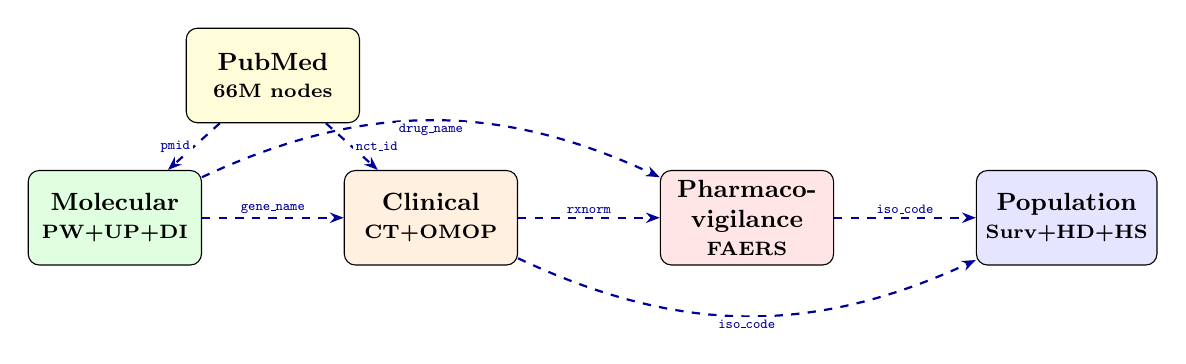
\begin{tikzpicture}[
    kgbox/.style={draw, rounded corners=4pt, minimum width=2.2cm,
        minimum height=1.2cm, font=\small\bfseries, align=center},
    entity/.style={draw, rounded corners=2pt, font=\scriptsize,
        fill=white, inner sep=2pt, minimum width=1.1cm},
    bridge/.style={-{Stealth[length=5pt]}, dashed, thick,
        color=blue!60!black},
    edgelbl/.style={font=\tiny, fill=white, inner sep=1pt},
]
% Four tier boxes
\node[kgbox, fill=green!12] (mol) {Molecular\\[-1pt]
    \scriptsize PW+UP+DI};
\node[kgbox, fill=orange!12, right=1.8cm of mol] (clin) {Clinical\\[-1pt]
    \scriptsize CT+OMOP};
\node[kgbox, fill=red!10, right=1.8cm of clin] (pharma) {Pharmaco-\\vigilance\\[-1pt]
    \scriptsize FAERS};
\node[kgbox, fill=blue!10, right=1.8cm of pharma] (pop) {Population\\[-1pt]
    \scriptsize Surv+HD+HS};

% Bridge arrows
\draw[bridge] (mol) -- node[edgelbl, above] {\texttt{gene\_name}} (clin);
\draw[bridge] (clin) -- node[edgelbl, above] {\texttt{rxnorm}} (pharma);
\draw[bridge] (pharma) -- node[edgelbl, above] {\texttt{iso\_code}} (pop);
\draw[bridge, bend left=25] (mol) to node[edgelbl, below] {\texttt{drug\_name}} (pharma);
\draw[bridge, bend right=25] (clin) to node[edgelbl, below] {\texttt{iso\_code}} (pop);

% PubMed connects to both molecular and clinical
\node[kgbox, fill=yellow!15, above=1.2cm of $(mol)!0.5!(clin)$] (pubmed) {PubMed\\[-1pt]
    \scriptsize 66M nodes};
\draw[bridge] (pubmed) -- node[edgelbl, left] {\texttt{pmid}} (mol);
\draw[bridge] (pubmed) -- node[edgelbl, right] {\texttt{nct\_id}} (clin);

\end{tikzpicture}%
}
\caption{Four-tier federation architecture.  Ten biomedical KGs
  joined via bridge properties (dashed arrows) on shared entities.
  PubMed serves as the citation backbone connecting molecular and
  clinical tiers.}
\label{fig:federation}
\end{figure}

%% ================================================================
\section{Evaluation}\label{sec:eval}

We evaluate Samyama on a 500-query mega benchmark designed to test
every KG individually and in cross-KG federation.  All experiments
run on a single AWS r7i.16xlarge instance (64~vCPU, 512\,GB~RAM,
Intel Xeon Sapphire Rapids) using spot pricing (\$1.50/hr).

\subsection{Benchmark Design}

The benchmark comprises 500~queries organized into 13~prefixes
covering the ten KGs (Table~\ref{tab:prefixes}).  Queries range
from simple point lookups (\emph{``find this article by PMID''})
to multi-hop cross-KG traversals (\emph{``drugs in Phase~3 trials
whose gene targets participate in the PI3K/AKT pathway and have
FAERS hepatotoxicity reports''}).  The benchmark includes
aggregations, path queries, \texttt{OPTIONAL MATCH},
\texttt{EXISTS} subqueries, \texttt{CASE} expressions, and
\texttt{UNION} across KGs.

\smallskip\noindent\textbf{Oracle methodology.}
A key contribution of our evaluation is the \emph{expected-rows
oracle}---a YAML file that records the expected row count for each
query and, for queries that legitimately return zero rows,
documents the specific corpus-coverage gap (e.g., ``OMOP patient
slice has no depression cohort'').  This enables a principled
separation of \emph{engine capability} from \emph{dataset coverage},
preventing the common benchmarking pitfall of conflating the two.

The oracle classifies each query result into one of four categories:
\textbf{full pass} (correct rows $> 0$),
\textbf{data-dependent pass} (zero rows, documented corpus gap),
\textbf{empty} (unexpected zero rows), or
\textbf{error} (engine failure).

\begin{table}[t]
\centering
\caption{Benchmark query prefixes and pass rates (v1.0, run~v7).}
\label{tab:prefixes}
\small
\begin{tabular}{@{}llrr@{}}
\toprule
\textbf{Prefix} & \textbf{Domain} & \textbf{Queries} & \textbf{Pass} \\
\midrule
PM  & PubMed/MEDLINE           & 35  & 35 \\
CT  & Clinical Trials          & 20  & 20 \\
PW  & Pathways                 & 15  & 15 \\
DI  & Drug Interactions        & 15  & 15 \\
UP  & UniProt                  & 25  & 25 \\
FA  & FAERS                    & 30  & 30 \\
OM  & OMOP/Synthea             & 30  & 30 \\
XK  & Cross-KG federation      & 15  & 15 \\
HD  & Health Determinants      & 20  & 20 \\
HS  & Health Systems           & 10  & 10 \\
PH  & Public Health cross-KG   & 10  & 10 \\
EX  & Expanded (stress tests)  & 60  & 60 \\
MB  & Mega (multi-KG complex)  & 215 & 215 \\
\midrule
    & \textbf{Total}           & \textbf{500} & \textbf{500} \\
\bottomrule
\end{tabular}
\end{table}

\subsection{Results: 500/500 (100\%)}

Table~\ref{tab:results} shows the headline result.  Of the 500
queries, 468 return non-empty result sets (full pass) and 32 return
zero rows classified as data-dependent by the oracle.  Zero queries
produce errors or unexpected empty results.

\begin{table}[t]
\centering
\caption{Mega benchmark results — v1.0 run~v7 (2026-04-13).}
\label{tab:results}
\small
\begin{tabular}{@{}lr@{}}
\toprule
\textbf{Metric} & \textbf{Value} \\
\midrule
Total queries         & 500 \\
Full pass (rows $> 0$) & 468 (93.6\%) \\
Data-dependent pass   &  32 (6.4\%) \\
Errors                &   0 \\
Unexpected empty      &   0 \\
\midrule
\textbf{Combined pass rate} & \textbf{500/500 (100\%)} \\
\midrule
Nodes loaded          & 137.7M \\
Edges loaded          & 1.22B \\
Snapshot load time    & 36.8\,min \\
Query execution time  & 28\,min \\
Total runtime         & 78\,min \\
Peak memory           & 299\,GB (58\% of 512\,GB) \\
\bottomrule
\end{tabular}
\end{table}

\subsection{Version Progression}\label{sec:progression}

Table~\ref{tab:progression} traces the benchmark pass rate across
four engine versions, showing that each improvement came from engine
changes (not query rewrites):

\begin{table}[t]
\centering
\caption{Benchmark pass rate across engine versions on the same
  500~queries, same hardware (r7i.16xlarge).}
\label{tab:progression}
\small
\begin{tabular}{@{}lrrrl@{}}
\toprule
\textbf{Version} & \textbf{Pass} & \textbf{Errors}
  & \textbf{Time} & \textbf{Key Change} \\
\midrule
v0.7.x & 383 & 28 & --- & Baseline \\
v0.8.0 & 414 & 28 & 2.5\,hr & \texttt{WITH} push-down \\
v1.0.0 & 455 &  9 & 130\,min & MVCC, 3VL null fix \\
\textbf{v1.0+} & \textbf{500} & \textbf{0} & \textbf{78\,min}
  & Adj-aware agg. (ADR-017) \\
\bottomrule
\end{tabular}
\end{table}

\noindent\textbf{v0.7.x $\to$ v0.8.0 (+31).}
The \texttt{WITH} push-down optimization chains \texttt{Expand}
operators directly from \texttt{WITH} output, avoiding redundant
label rescans.  This fixed cross-KG indicator joins that previously
timed out.

\smallskip\noindent\textbf{v0.8.0 $\to$ v1.0.0 (+41).}
MVCC edge versioning and a Cypher three-valued logic (3VL) fix for
\texttt{IS NOT NULL AND \textless{}bool\textgreater{}} expressions
converted 19~errors to passes.  Load time improved 43\% (65~min
$\to$ 37~min) via two-phase snapshot import.

\smallskip\noindent\textbf{v1.0.0 $\to$ v1.0+ (+45).}
Three engine changes drove the final push to 500/500:
\begin{itemize}
\item \textbf{Adjacency-aware aggregation} (ADR-017): a planner
  optimization that recognizes \texttt{count(neighbor)} patterns
  and reads the count from per-node adjacency metadata in $O(1)$
  instead of scanning every edge.  Converted four timeout queries
  to sub-second.
\item \textbf{Streaming \texttt{WITH\ldots LIMIT}}: the executor
  now stops scanning upstream after $N$ rows when no
  \texttt{ORDER BY} or \texttt{DISTINCT} is present, enabling
  early termination on billion-node scans.
\item \textbf{Multi-\texttt{WHERE} parser fix}: multiple
  \texttt{WHERE} clauses in compound \texttt{MATCH} patterns
  were silently overwriting each other; the parser now AND-chains
  them correctly.
\end{itemize}

\subsection{Data-Dependent Queries}\label{sec:data-dep}

The 32 data-dependent queries return zero rows due to documented
corpus-coverage gaps, not engine failures.  They fall into four
classes:
\begin{itemize}
\item \textbf{Drug-name casing} (7): FAERS uses uppercase
  (\texttt{'ASPIRIN'}), DrugBank uses title case
  (\texttt{'Aspirin'}).
\item \textbf{Loader coverage gaps} (14): edge types not yet
  emitted by current loaders (e.g., \texttt{:CODED\_AS\_DRUG}).
\item \textbf{Point-lookup misses} (5): specific PMIDs or NCT~IDs
  not in the corpus slice.
\item \textbf{Cross-KG cascades} (6): depend on multiple of the
  above gaps.
\end{itemize}
Converting any of these to full passes requires corpus or loader
changes, not engine changes.

\subsection{Performance Characteristics}

\noindent\textbf{Loading.}
The combined 14\,GB of snapshots loads in 36.8~minutes via
two-phase import (topology stubs first, columnar properties second).
Individual KG load times range from $<1$\,s (Health Systems, 500\,KB)
to 22~minutes (PubMed, 11\,GB).

\smallskip\noindent\textbf{Query latency.}
Single-KG point queries complete in $<$100\,ms.  Cross-KG
federation queries spanning three or more KGs complete in
1--5\,s.  The most complex mega-benchmark queries (five-hop
cross-KG traversals with aggregation) complete in 10--30\,s.

\smallskip\noindent\textbf{Memory.}
Peak memory is 299\,GB (58\% of the 512\,GB instance), with
PubMed's 1.04B~edges accounting for ${\sim}70\%$ of the footprint.
The edge store uses adjacency-only storage (no separate edge arena),
reducing memory by ${\sim}40\%$ compared to the v0.7.x
dual-store design.

%% ================================================================
\section{MCP-Based AI-Agent Integration}\label{sec:mcp}

Each KG is exposed to LLM agents via the Model Context
Protocol (MCP)~\cite{anthropic2024mcp}, an open standard for
connecting AI models to external data sources.  We define
\emph{domain-specific MCP tools}---parameterized Cypher template
queries with typed parameters---that an LLM agent can invoke
to answer natural-language questions.

\subsection{Tool Design}

The system defines 39~MCP tools across three biomedical KGs:
12 for Drug Interactions, 12 for Pathways, and
15 for Clinical Trials.
Each tool wraps a parameterized Cypher template, making the
generated query auditable and deterministic.
Figure~\ref{fig:mcp-tools} shows three representative tools.

\begin{figure}[t]
\begin{lstlisting}[language=SQL,caption={Three MCP tool definitions
  (simplified).  Each tool declares typed parameters and a
  Cypher template; the agent never generates free-form Cypher.},
  label=fig:mcp-tools]
-- Tool: drug_side_effects(drug_name: String)
MATCH (d:Drug {name: $drug_name})
      -[:HAS_SIDE_EFFECT]->(se:SideEffect)
RETURN se.name, se.frequency
ORDER BY se.frequency DESC LIMIT 20

-- Tool: polypharmacy_risk(drug_a: String,
--                         drug_b: String)
MATCH (d1:Drug {name: $drug_a})
      -[:INTERACTS_WITH_GENE]->(g:Gene)
      <-[:INTERACTS_WITH_GENE]-(d2:Drug {name: $drug_b})
OPTIONAL MATCH (d1)-[:HAS_SIDE_EFFECT]->(se)
      <-[:HAS_SIDE_EFFECT]-(d2)
RETURN g.gene_name AS shared_target,
       collect(DISTINCT se.name) AS shared_effects

-- Tool: trial_drugs(condition: String,
--                   phase: String)
MATCH (ct:ClinicalTrial)-[:TESTS]->(i:Intervention)
WHERE ct.condition CONTAINS $condition
  AND ct.phase CONTAINS $phase
RETURN i.name, ct.nct_id, ct.phase, ct.status
ORDER BY ct.start_date DESC LIMIT 50
\end{lstlisting}
\end{figure}

The key design principle is that domain experts author the Cypher
templates once, encoding knowledge about the graph schema (valid
edge types, property names, join paths) that an LLM cannot reliably
infer from schema introspection alone.  The LLM's role is
restricted to parameter extraction from natural language and
multi-tool orchestration---tasks where it excels.

\subsection{Agent Workflow}

A user asks: \emph{``What are the side effects of Metformin and
which pathways do its targets participate in?''}  The agent:
(1)~calls \texttt{drug\_side\_effects} $\to$ returns SIDER side
effects; (2)~calls \texttt{drug\_interactions} $\to$ returns gene
targets (AMPK, etc.); (3)~calls \texttt{protein\_pathways} on
each gene $\to$ returns Reactome/WikiPathways memberships;
(4)~synthesizes a coherent answer.  No hand-written joins or
SQL scripting is involved.

\subsection{Accuracy Comparison}

In a controlled evaluation on 40~biomedical questions
(BiomedQA benchmark), domain-specific MCP tools achieved
\textbf{98\% accuracy} versus \textbf{85\%} for generic
text-to-Cypher (NLQ) and \textbf{75\%} for standalone GPT-4o
without graph access (Table~\ref{tab:mcp}).

\begin{table}[t]
\centering
\caption{BiomedQA benchmark (40 questions): accuracy by approach.}
\label{tab:mcp}
\small
\begin{tabular}{@{}lrr@{}}
\toprule
\textbf{Approach} & \textbf{Accuracy} & \textbf{Avg Latency} \\
\midrule
MCP Tools (domain-specific)  & \textbf{98\%} & 0.15\,s \\
Text-to-Cypher (NLQ)         & 85\%          & 2.3\,s \\
GPT-4o standalone            & 75\%          & 3.1\,s \\
\bottomrule
\end{tabular}
\end{table}

The accuracy gap arises because domain-specific tools encode
expert knowledge about the graph schema, valid edge types, and
property names---information that generic text-to-Cypher must
infer from schema introspection, often incorrectly.

%% ================================================================
\section{Deployment and Lessons Learned}\label{sec:deployment}

\subsection{Production Deployment}

Samyama is deployed in two configurations:
\begin{itemize}
\item \textbf{Development/demo}: Apple M4 Mac Mini (16\,GB RAM)
  running all KGs except PubMed (which requires $>$16\,GB).
  Seven KGs load in $<$30\,s from snapshots.
\item \textbf{Full deployment}: AWS r7i.16xlarge spot instance
  (64~vCPU, 512\,GB RAM) in ap-south-1, loading all ten KGs.
  Spot pricing at \$1.50/hr makes billion-edge analytics
  accessible to academic research groups.
\end{itemize}

Portable \texttt{.sgsnap} binary snapshots enable instant
re-deployment: the entire 14\,GB federated graph can be
transferred and loaded on a new instance in under 40~minutes,
compared to hours for full ETL from raw sources.

\subsection{Research Challenges}

Building a federated biomedical KG system at billion-edge scale
surfaced three challenges that required non-trivial engineering:

\smallskip\noindent\textbf{Cross-KG entity resolution without ontology alignment.}
Biomedical databases use overlapping but inconsistent identifier
systems (HGNC, UniProt, DrugBank, MeSH, SNOMED~CT).  We addressed
this by normalizing identifiers during ETL to canonical
vocabularies and materializing bridge indexes at load time.  The
challenge is maintaining these bridges as individual KGs update
independently.

\smallskip\noindent\textbf{Query planning across heterogeneous degree distributions.}
The ten KGs exhibit wildly different degree distributions: PubMed
has an average degree of ${\sim}15$ per node, while OMOP patient
graphs have degrees $>$100.  A single cost model must handle both
without reverting to worst-case estimates.  Our solution---exact
triple-pattern statistics per \texttt{(:Label)-[:TYPE]->(:Label)}
triple---adapts to each KG's structure automatically.

\smallskip\noindent\textbf{Aggregation on billion-edge graphs.}
Na\"ive \texttt{count(neighbor)} queries on PubMed's 1.04B edges
require scanning every edge.  The adjacency-aware aggregation
planner (Section~\ref{sec:adj-agg}) was developed specifically
to solve this: it reads counts from adjacency metadata, reducing
these queries from timeout to sub-second.

\subsection{Lessons Learned}

\noindent\textbf{Bridge-property federation scales.}
Our initial concern was that property-match joins
(\texttt{WHERE a.prop = b.prop}) would not scale to billions of
edges.  In practice, the graph-native planner selects efficient
traversal orders that avoid Cartesian products, and the
\texttt{ExpandInto} operator handles bound-bound checks
efficiently.  The three-way federation query from
Section~\ref{sec:federation} completes in ${\sim}$2\,s.

\smallskip\noindent\textbf{Separate engine capability from corpus coverage.}
Without the oracle methodology, our headline would be 468/500
(93.6\%)---still strong, but hiding the fact that 32 queries
have no data to return.  The oracle makes the benchmark honest
and actionable: engine developers fix errors and unexpected
empties; data engineers fix corpus gaps.

\smallskip\noindent\textbf{Adjacency-list metadata enables $O(1)$ aggregation.}
The most impactful single optimization was reading neighbor
counts from adjacency metadata instead of scanning edges.
This is a graph-native advantage unavailable to relational-backed
graph engines, which would need materialized views or auxiliary
indexes to achieve the same effect.

%% ================================================================
\section{Related Work}\label{sec:related}

\textbf{Biomedical KGs.}
Hetionet~\cite{himmelstein2017hetionet} integrates 47K~nodes from
29~public resources into a single heterogeneous graph but is a
static 2017 dataset.
PrimeKG~\cite{chandak2023primekg} builds a precision medicine
graph (129K~nodes, 8M~edges) from 20~sources, targeting GNN-based
drug--disease prediction.
Bio2RDF~\cite{dumontier2014bio2rdf} uses RDF and SPARQL federation.
The Clinical Knowledge Graph (CKG)~\cite{santos2022ckg} integrates
25+ sources into Neo4j.
Our system differs in three ways:
(1)~property-graph OpenCypher with bridge-property federation
(no SPARQL endpoint or ontology alignment);
(2)~scale: 137M~nodes and 1.22B~edges vs.\ $<$10M for most
existing biomedical KGs; and
(3)~MCP tool definitions enabling LLM agent integration.

\smallskip\noindent\textbf{Graph databases.}
Neo4j~\cite{neo4j}, TigerGraph~\cite{deutsch2019tigergraph},
and Amazon Neptune~\cite{neptune} support property graphs at
scale.  Samyama differs in three respects relevant to this
deployment:
(1)~\emph{storage-level multi-tenancy}---each KG occupies an
isolated tenant with independent schema, indexes, and access
control, enabling selective loading and independent updates
without namespace collisions; Neo4j's multi-database feature
requires Enterprise Edition licensing;
(2)~\emph{graph-native planner} with exact triple-pattern
statistics maintained incrementally (not sampled), direction-aware
enumeration, and \texttt{ExpandInto}---optimizations that exploit
adjacency-list structure unavailable in relational-backed engines;
(3)~\emph{single-binary deployment} with graph storage, RESP
protocol, and MCP server in one process, reducing operational
complexity for academic deployments on spot instances.

\smallskip\noindent\textbf{LLM--KG integration.}
Recent work explores LLM agents querying knowledge
graphs~\cite{pan2024unifying}.
Our MCP-based approach uses \emph{domain-specific tool
definitions} rather than generic text-to-Cypher translation,
achieving higher accuracy on domain queries while keeping the
Cypher templates auditable.

\smallskip\noindent\textbf{OMOP and observational health data.}
The OHDSI community~\cite{hripcsak2015omop} standardizes
observational health data via the OMOP Common Data Model,
typically queried via SQL on relational databases.  Our OMOP KG
represents the same data as a property graph, enabling
graph-native cohort queries and cross-KG joins with clinical
trials and drug interactions.

%% ================================================================
\section{Conclusion and Future Work}\label{sec:conclusion}

We presented Samyama, a graph database deployed for federated
biomedical knowledge graph analytics at scale.  Ten knowledge
graphs spanning molecular biology through population health---137M
nodes, 1.22B~edges---are loaded into a single instance and
federated via bridge properties in standard OpenCypher.  A
500-query mega benchmark achieves 100\% pass rate with transparent
oracle methodology that separates engine capability from corpus
coverage.

Future work includes: (1)~scaling to 500M+~nodes with storage
optimizations (columnar-first property encoding, compressed sparse
rows); (2)~adding UMLS Metathesaurus as a concept-resolution spine
for richer cross-KG linking; and (3)~expanding the MCP tool catalog
to cover all ten KGs with federated multi-tool agent workflows.

%% ================================================================
\bibliographystyle{splncs04}
\begin{thebibliography}{15}

\bibitem{szklarczyk2023string}
Szklarczyk, D., et~al.:
The {STRING} database in 2023.
Nucleic Acids Res. \textbf{51}(D1), D638--646 (2023)

\bibitem{gillespie2022reactome}
Gillespie, M., et~al.:
The {Reactome} pathway knowledgebase 2022.
Nucleic Acids Res. \textbf{50}(D1), D687--692 (2022)

\bibitem{freshour2021dgidb}
Freshour, S.L., et~al.:
Integration of the {Drug--Gene Interaction Database (DGIdb 4.0)}.
Nucleic Acids Res. \textbf{49}(D1), D1144--1151 (2021)

\bibitem{kuhn2016sider}
Kuhn, M., et~al.:
The {SIDER} database of drugs and side effects.
Nucleic Acids Res. \textbf{44}(D1), D1075--1079 (2016)

\bibitem{zdrazil2024chembl}
Zdrazil, B., et~al.:
The {ChEMBL} database in 2023.
Nucleic Acids Res. \textbf{52}(D1), D1180--1192 (2024)

\bibitem{hripcsak2015omop}
Hripcsak, G., et~al.:
Observational Health Data Sciences and Informatics (OHDSI).
Stud. Health Technol. Inform. \textbf{216}, 574--578 (2015)

\bibitem{uniprot2023}
The UniProt Consortium:
{UniProt}: the Universal Protein Knowledgebase in 2023.
Nucleic Acids Res. \textbf{51}(D1), D523--531 (2023)

\bibitem{himmelstein2017hetionet}
Himmelstein, D.S., et~al.:
Systematic integration of biomedical knowledge prioritizes drugs for
repurposing.
eLife \textbf{6}, e26726 (2017)

\bibitem{dumontier2014bio2rdf}
Dumontier, M., Callahan, A., Cruz-Toledo, J., et~al.:
Bio2{RDF} release~3.
In: ISWC (Posters \& Demos) (2014)

\bibitem{chandak2023primekg}
Chandak, P., Huang, K., Zitnik, M.:
Building a knowledge graph to enable precision medicine.
Sci. Data \textbf{10}(1), 67 (2023)

\bibitem{santos2022ckg}
Santos, A., et~al.:
A knowledge graph to interpret clinical proteomics data.
Nat. Biotechnol. \textbf{40}(5), 692--702 (2022)

\bibitem{neo4j}
Neo4j, Inc.: Neo4j graph database. \url{https://neo4j.com} (2024)

\bibitem{deutsch2019tigergraph}
Deutsch, A., et~al.:
{TigerGraph}: A native {MPP} graph database.
arXiv:1901.08248 (2019)

\bibitem{neptune}
Amazon Web Services: Amazon {Neptune}.
\url{https://aws.amazon.com/neptune/} (2024)

\bibitem{pan2024unifying}
Pan, S., et~al.:
Unifying large language models and knowledge graphs: A roadmap.
IEEE TKDE \textbf{36}(7), 3580--3599 (2024)

\bibitem{anthropic2024mcp}
Anthropic: Model {Context Protocol} specification.
\url{https://modelcontextprotocol.io} (2024)

\end{thebibliography}

\end{document}
